\stepcounter{lecture}
\setcounter{lecture}{3}

\pagebreak

\sektion{Continuity}

\subsektion{Continuity and Limits}
\begin{definition}
	Given a function $f: \RR \to \RR$, we say that $f$ is \emph{continuous at $a \iR$} if and only if 
	\[\forall \epsilon >0, ~\exists \delta >0 \text{ such that } |x-a| < \delta \implies |f(x) - f(a)| < \epsilon \]
\end{definition}

So $\delta$ depends on $a, \epsilon$. ``Once $x$ is close to $a$, then $f(x)$ is close to $f(a)$''.

More precisely: ``However close (i.e. within $\epsilon$) I want $f(x)$ to be to $f(a)$, I can arrange it by taking $x$ close (i.e. within $\delta$) to $a$''.


\begin{center}
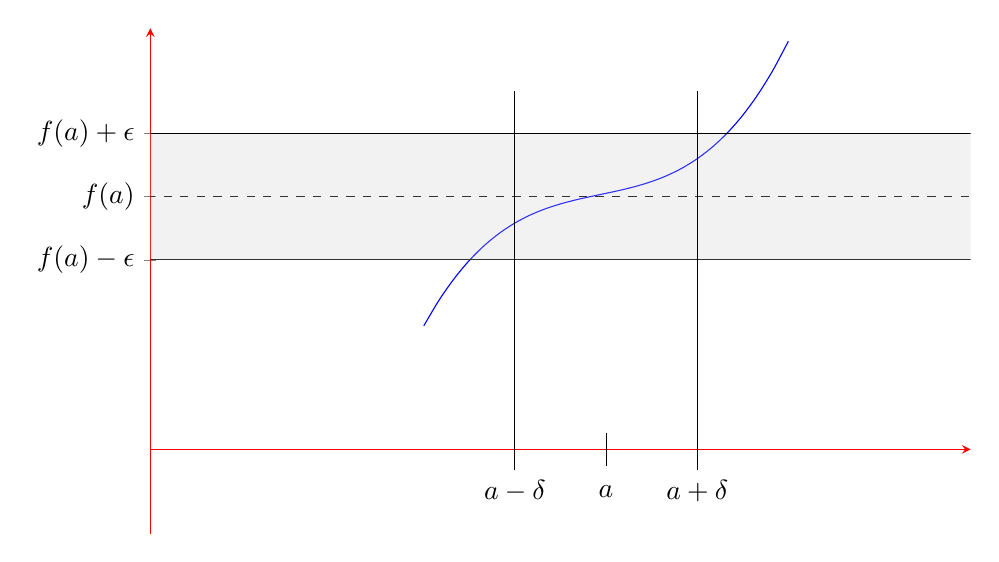
\begin{tikzpicture}
\begin{axis}[
 axis line style={red},
 axis lines=middle,
   %  x label style={at={(axis description cs:1.05,0.4)}},
   %  y label style={at={(axis description cs:-0.08,1.02)}},
  ymin = -0.2,
  ymax = 1,
  xmin = 1,
  xmax = 10,
     ytick = {0.75, 0.45,0.6},
   yticklabels={$f(a) + \epsilon$,$f(a) -\epsilon$, $f(a)$},
   xtick = 0,
  width=12cm,height=8cm]
   \addplot[draw=blue, domain=4:8,smooth] {(0.0309*x^3 - 0.5504*x^2 + 3.313*x - 6.13)};
       \draw (axis cs:20,0.75) -- (axis cs:0,0.75); %fa+e line
      \draw (axis cs:20,0.45) -- (axis cs:0,0.45); %fa-e line
       \draw[dashed] (axis cs:20,0.6) -- (axis cs:0,0.6); %fa line
         \fill[gray!40,nearly transparent] (axis cs:0,.45)-- (axis cs: 0,0.75) -- (axis cs: 10,0.75) -- (axis cs: 10,0.45) -- cycle;
            \draw (axis cs:5,0.85) -- (axis cs:5,-0.05) node at (axis cs:5,-0.1) {$a-\delta$};
                        \draw (axis cs:6,0.04) -- (axis cs:6,-0.04)  node at (axis cs:6,-0.1) {$a$};
                        \draw (axis cs:7,0.85) -- (axis cs:7,-0.05) node at (axis cs:7,-0.1) {$a + \delta$};
  \end{axis}
\end{tikzpicture}
\end{center}


Equivalently: $\forall \epsilon > 0,~ \exists \delta >0 \text{ such that } |f(x) - f(a)| < \epsilon ~ \forall x \text{ with } |x-a| < \delta$\\

Or: $\forall \epsilon > 0, ~ \exists \delta > 0 \text{ such that } f(a- \delta, a + \delta) \subseteq (f(a)- \epsilon, f(a) + \epsilon)$

Where $S\subseteq R$ then $f(S)$ is the set $\{f(x):x \in S\}$\\

Or: $\forall \epsilon,~\exists \delta >0 \text{ such that } f^{-1}(f(a) - \epsilon, f(a) + \epsilon) \supseteq (a - \delta, a + \delta)$

Where $f: A \to B \subset T$ then $f^{-1}(T) = \{a \in A:f(a) \in T\}$ [Don't need $f^{-1}$ to exist !!]\\


\begin{example}
\[f(x) = \begin{cases}
 0 & x \leq 0 \\
 1 & x > 0	
 \end{cases}
\]	 Then $f$ is not continuous at $x = 0$

\begin{proof}
Take $\epsilon = 1$ (or $0 < \epsilon < 1$). Then if $f$ is continuous at $x = 0$ we know that $\exists \delta > 0$ such that $|f(x) - f(0)| < 1~ \forall x \in (0 - \delta, 0 + \delta)~(*)$. In particular, take $x = \delta/2$ to find that $|1-0| < 1$ by 	$(*)$.
\end{proof}
\end{example}

``Jump discontinuity'' is another type of discontinuity\\


\begin{example}
\[f(x) = \begin{cases}
 \sin(\frac{1}{x}) & x \neq 0\\
 r & x = 0	
 \end{cases}
\] Then $f$ is discontinuous at $x = 0$ (for any $r$).	

\begin{center}
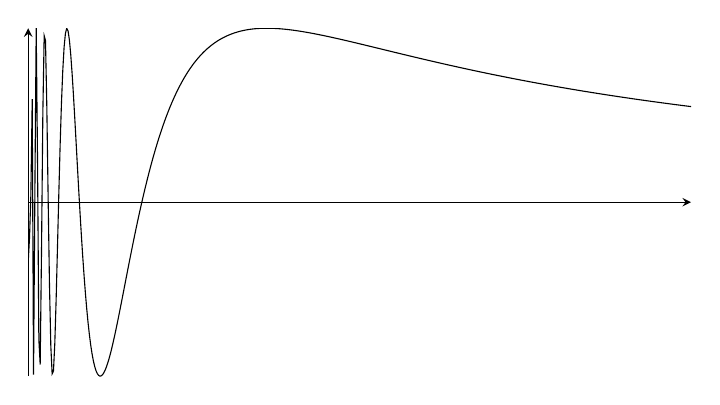
\begin{tikzpicture}
\begin{axis}[
axis lines=middle,
xtick = 0,
ytick = 0,
  width=10cm,height=6cm]
   \addplot[domain=0.0005:0.03,samples=500]{sin(1/x)};
 \end{axis}
\end{tikzpicture}
\end{center}

\emph{Idea of proof}: If $f$ is continuous at $x = 0$, then $f(x) \in (r-\epsilon, r + \epsilon)$ is close to $f(0) = r$ for $x \in (- \delta, \delta).$ In particular, $f(x)$ and $f(y)$ are close to each other (within $2\epsilon$). But $f(x)$ could be $+1$ and $f(y)$ could be $-1$, $\cont$.
\begin{proof}
Fix $\epsilon \in (0,1]$. If $f$ is continuous at $0$, then $\exists \delta > 0$ such that $|f(x) - f(0)| < \epsilon~\forall x \in (\delta,\delta)$. In particular, $\forall x,y \in (-\delta, \delta), |f(x) - f(y)| < 2\epsilon \leq 2$, by the triangle inequality. 

Now choose $n \in \mathbb{N}$, $n > \frac{1}{\delta}$. Then take $x = \frac{1}{(4n+1)\pi/2} \in (0,\delta)$, $y = \frac{1}{(4n+3)\pi/2} \in (0,\delta)$. Then 
\[|\sin(1/x) - \sin(1/y)| = |1 - (-1)| = 2 ~\cont\qedhere\]
\end{proof}

\end{example}~


\begin{example}
\lecturemarker{18}{5 Oct}
$f: \RR \to \RR$, $f = mx + c$ is continuous at $a, ~\forall a \iR$. 

\emph{Rough working:} We want 
\[\begin{aligned}|f(x) - f(a)| < \epsilon &\iff |(mx+c) - (ma + c)|  < \epsilon \\
&\iff |mx(-a)| < \epsilon\\
&\iff |x-a| < \frac{\epsilon}{|m|} \text{ if } m \neq 0 \\
&\impliedby |x-a| < \frac{\epsilon}{|m|+1} 
\end{aligned}
\]
So set $\delta:= \epsilon / (1 + |m|)$. Then $|x-a| < \delta \implies |f(x) - f(a)| < \epsilon$
\begin{proof}
Set $\delta:= \frac{\epsilon }{1 + |m|} > 0$. Then when $|x-a| < \delta$ we have  
\[\begin{aligned}
|(mx+ c) - (ma +c)| &= |f(x) - f(a)| \\
&= |m||x-a| \\
&< |m|\delta = \epsilon \frac{|m|}{|m|+1} < \epsilon	
\end{aligned}\]
\end{proof}
\end{example}

\begin{example}
$f: \RR\to \RR, f(x) = x^2$
Proposition: $f$ continuous on $\RR$ (i.e. at $a,~\forall a \iR$)

\emph{Rough working:} 
\[|f(x) - f(a)| = |x^2-a^2| = |x+a||x-a|\]
we want this to be $< \epsilon$, i.e. $|x-a| < \frac{\epsilon}{|x+a|} *(*)$

But we can't let $\delta$ depend on $x$!!

\textbf{Problem:} If $|x-a| < \frac{\epsilon}{R} \forall R>0$, then $|x-a| =0$.

\textbf{Solution:} I only care about $x$ close to $a$; within $1$ say.


So, so long as I choose $\delta \leq 1$, then I know that 
\[|x-a| < \delta \implies |x+a| \leq |x-a| + 2|a| \leq 1 + 2|a|\]
So now $|x-a| < \dfrac{\epsilon}{1 + 2|a|} \implies (*)$

So to ensure both conditions we set $\delta = \mathrm{min}\{1,\epsilon/(1+2|a|)\}$

\begin{proof}
Fix $\epsilon >0$, $a \iR$. Set $\delta = \mathrm{min}\{1,\frac{\epsilon}{1 + 2|a|}\}$. Then $|x-a| < \delta \implies$
\begin{enumerate}
\item $|x-a| < 1 \implies |x+a| < 1 + 2|a|$
\item $|x-a| < \dfrac{\epsilon}{1 + 2|a|}$
\end{enumerate}

\[\implies |x^2 -a^2| = |x-a||x+a| < \dfrac{\epsilon}{1+2|a|}\cdot(1+2|a|) = \epsilon\]
\end{proof}
\end{example}~

\begin{clicker}
Fix $a,b \iR$. Then $x < a \implies x < b$ tells us? 

\textbf{Answer:} $a \geq b$. 

Prove that $f(x) = \begin{cases}
 	\frac{1}{x} & x \neq 0\\
 	0 & x = 0
 \end{cases}$
 is discontinuous at $x = 0$

Student answer:
\begin{enumerate}
\item Suppose $f$ is cts at $0$
\item Then $\forall \epsilon >0,~\exists \delta > 0$ s.t.
\item $|x| < \delta \implies |f(x) - f(0)| = |1/x| < \epsilon$
\item $\implies |1/(x/2)| = |2/x| < 2\epsilon$
\item But $|x| < \delta \implies |x/2| < \delta$ so
\item should get that $|f(x/2) - f(0)| = |1/(x/2)| < \epsilon$
\item This contradicts $(*)$	
\item So $f$ is not continuous at $0$
\end{enumerate}

\textbf{Answer:} (vii) is the problem. (vi) $\implies$ (iv) doesn't contradict (iv).
\end{clicker}


Notice 
\lecturemarker{19}{5 Oct} the definition of continuity makes sense whenever I have a notion of distance.  e.g. in $\RR^n$ use $|\vec{x} - \vec{y}| := \sqrt{\sum_{i=1}^n (x_i - y_i)^2}$.\\

\begin{definition}
$f: \RR^n \to \RR^m$ is continuous at $a \in \RR^n$ iff 
\[\forall \epsilon >0,~\exists \delta >0 \text{ s.t. } |\vec{x} - \vec{a}| < \delta \implies |f(\vec{x}) - f(\vec{a})| < \epsilon\]	
\end{definition}

\textbf{Notation:} The $\epsilon$-ball around $\vec{a}\in\RR^n$ is $B_\epsilon(\vec{a}) := \{\vec{x} \in \RR^n |\vec{x} - \vec{a}| < \epsilon\}$

So if $n = 1$, $B_\epsilon(a) = (a-\epsilon, a + \epsilon) \subseteq \RR$. 

Using this we can rewrite our definition of continuity:\\

\begin{definition}
$f: \RR^n \to \RR^m$ is continuous at $\vec{a} \in \RR^n$ iff 
\[\forall \epsilon > 0,~\exists \delta > 0 \text{ s.t. } f(B_\delta(\vec{a})) \subseteq B_\epsilon(f(\vec{a}))\]	
\end{definition}

So every point within $\delta$ of $\vec{a}$ gets mapped by $f$ to within $\epsilon$ of $f(\vec{a})$, equivalently 
\[\boxed{\forall \epsilon > 0,~\exists \delta > 0 \text{ s.t. } B_\epsilon(\vec{a}) \subseteq f^{-1}(B_\epsilon(f(\vec{a})))}\]


\begin{center}
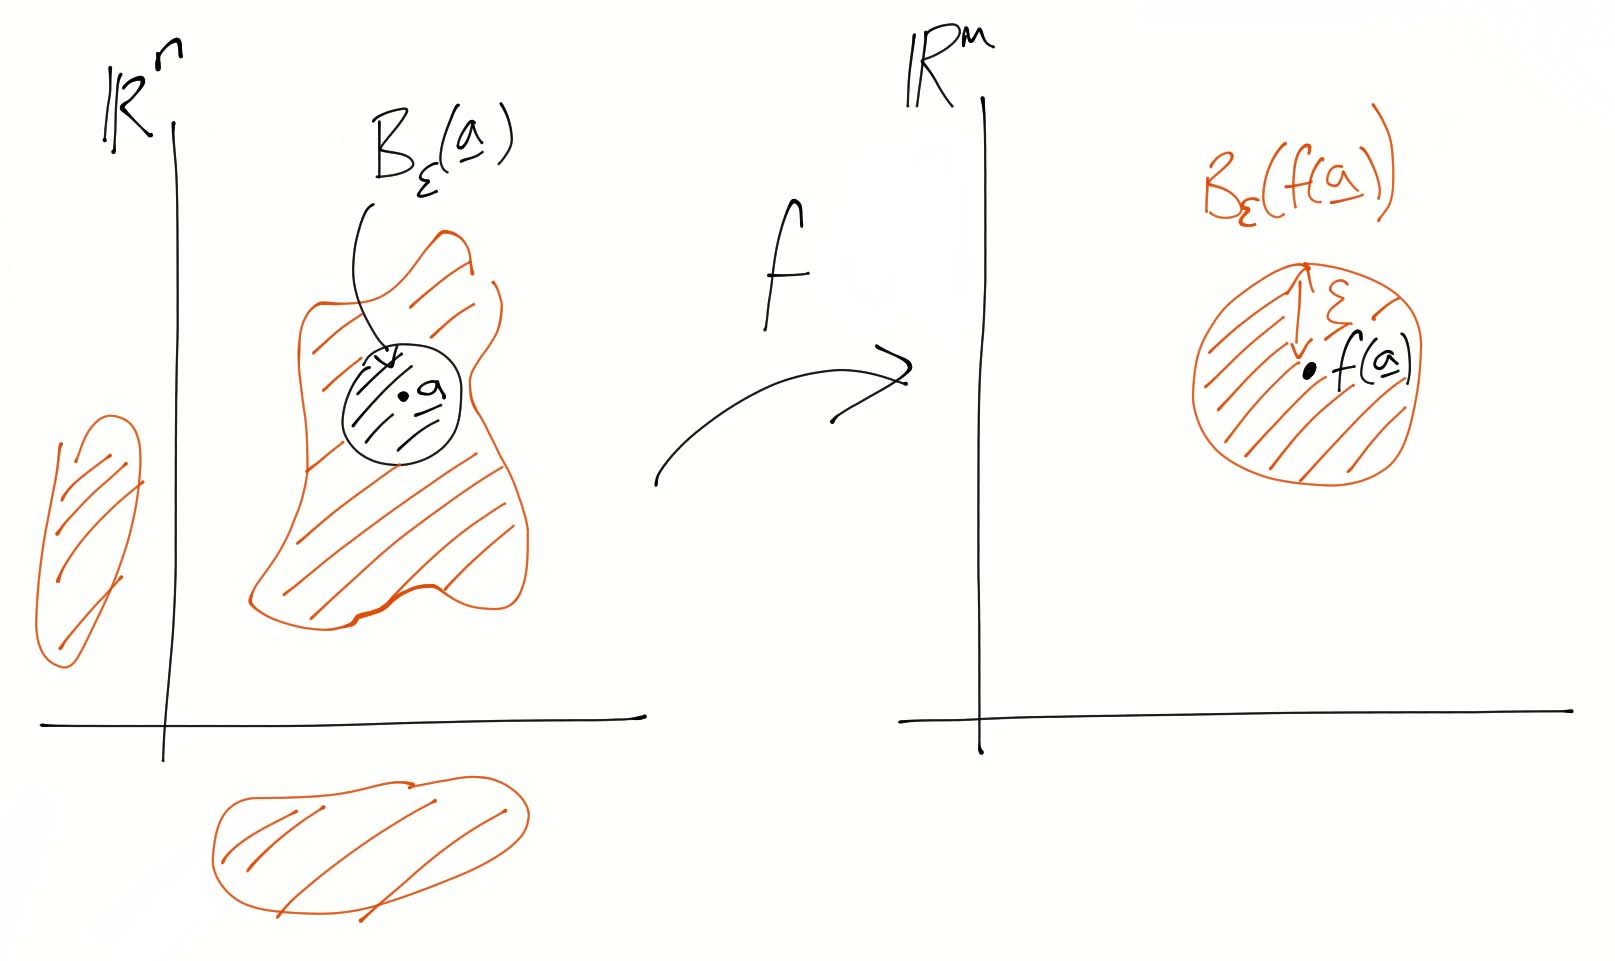
\includegraphics[width = 12cm]{ball1.jpg}
\end{center}


$f^{-1}(B_\epsilon(f(\vec{a}))) := \{\vec{x} \in \RR^n : f(\vec{x}) \in B_\epsilon (f(\vec{a}))\}$

Continuity at $\vec{a}$ says that $\vec{a}$ is in the ``interior'' of $f^{-1}(B_\epsilon (f(\vec{a})))$, i.e. $\exists$ a small ball $B_\delta (\vec{a})$ around it which is also in $f^{-1}(B_\epsilon(f(\vec{a})))$. 

So continuity at $\vec{a} \iff$ If $\vec{x}$ moves a tiny bit around $\vec{a}$ then $f(\vec{x})$ moves a tiny bit around $f(\vec{a})$.\pagebreak

\begin{example}
$f(x) = \begin{cases}
 	x\sin 1/x & x \neq 0\\
 	0 & x = 0
 \end{cases}$

\begin{center}
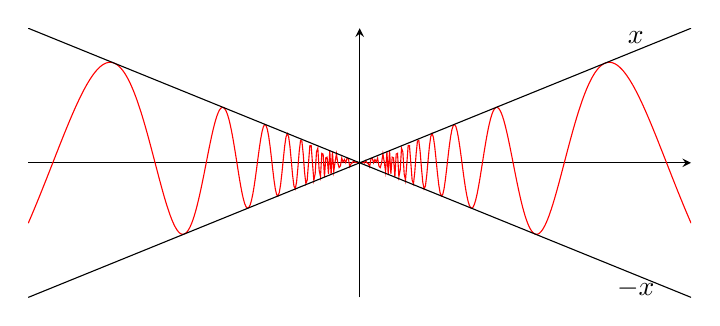
\begin{tikzpicture}
\begin{axis}[
axis lines=middle,
xtick = 0,
ytick = 0,
  width=10cm,height=5cm]
   \addplot[color = red, domain=-0.003:0.003,samples=500]{x*sin(1/x)};
   \addplot[domain=-0.003:0.003,smooth]{x};
   \addplot[domain=-0.003:0.003,smooth]{-x};
   \draw node at (axis cs: 0.0025,0.0028) {$x$};
   \draw node at (axis cs: 0.0025,-0.0028) {$-x$};
 \end{axis}
\end{tikzpicture}
\end{center}


\begin{proposition}
$f$ is continuous at $0$	
\end{proposition}

\begin{proof}
Fix $\epsilon >0$. Then 
\[|f(x) - f(0) = |x\sin\frac{1}{x}| \leq |x|\]
Take $\delta = \epsilon$. Then $|x| < \delta \implies |x| < \epsilon \implies |f(x) - f(0)| < \epsilon$	
\end{proof}
\end{example}\vspace*{5pt}

\begin{proposition}
$E: \CC \to \CC$ defined by $E(z) := \sum_{n=0}^{\infty} \frac{z^n}{n!}$ is continuous (i.e. continuous at $a,~\forall a \iC$)	
\end{proposition}
[Ex: from this show that $x \mapsto \sin x$ is continuous on $\RR$]

\emph{Rough working:} 
\[\begin{aligned}
|E(z) - E(a)| &= |E(a)(E(z-a)-E(0))| \\ 	
&= |E(a)| |E(z-a) -1|\\
& \leq |E(a)| \cdot \frac{|z-a|}{1-|z-a|}
\end{aligned}
\]
for $|z-a| < 1$ (see earlier lecture)
\[\begin{aligned}
\text{We want this to be } < \epsilon &\iff |z-a| < \frac{\epsilon}{|E(a)|}(1-|z-a|)\\
&\iff (1 + \epsilon/|E(a)|)|z-a| < \frac{\epsilon}{|E(a)|}\\
&\iff |z-a| < \epsilon/|E(a)|/(1 + \epsilon/|E(a)|)
\end{aligned}
\]


\begin{proof}
Fix $\epsilon >0$. Set $\delta = \dfrac{\epsilon}{|E(a)| + \epsilon} ~(*)$

Then we calculate that 
\[\begin{aligned}
|E(z) - E(a)| &\leq |E(a)| \frac{|z-a|}{1-|z-a|} \\
&< |E(a)| \cdot \frac{\delta}{1-\delta}	
\end{aligned}
\]	
for all $z$ with $|z-a| < \delta$. But by $(*)$, $\dfrac{\delta}{1-\delta} = \dfrac{\epsilon}{|E(a)|}$. 

So $|z-a|< \delta \implies |E(z) - E(a)| < \epsilon$.
\end{proof}~


\begin{theorem}
$f,g: \RR \to \RR$ cts at $a \in \RR \implies (f + g), f\cdot g$ are cts at $a$.
\end{theorem}
\begin{proof}
	Fix $\epsilon >0.$ \[\exists \delta_1 >0 \text{ such that }|x-a| < \delta_1 \implies |f(x) - f(a)| < \epsilon\] and\[\exists \delta_2 >0 \text{ such that }|x-a| < \delta_1 \implies |g(x) - g(a)| < \epsilon\]
	 Set $\delta =$ min$\{\delta_1,\delta_2\}.$ Then $\forall x$ such that $|x-a| < \delta:$
	\[|(f+g)(x) - (f+g)(a)| \leq |f(x) - f(a)| + |g(x) - g(a)| < 2\epsilon\]
	
	For (2): Similarly
	\[|f(x)g(x) - f(a)g(a)| \leq |g(x)||f(x) - f(a)| + |f(a)||g(x) - g(a)| ~(*)\]
	
	We need a bound on $|g(x)|$. We cannot bound $g(x)~ \forall x$!  But near $a$, $g(x)$ is close to $g(a)$, so we can bound $g(x)$ near $a$
	
	Take $\epsilon =1$ 
	\[\exists \delta_1 > 0\text{ s.t. }|x-a| < \delta_1 \implies |g(x) - g(a)| < 1 \implies |g(x)| < 1 + |g(a)| ~(A)\]
	
	Now fix any $\epsilon >0$. Then 
	\[\exists \delta_2 > 0\text{ s.t. }|x-a| < \delta_2 \implies |f(x) - f(a)| < \epsilon/1+|g(a)| ~ (B)\] (to cancel $|g(x)| < 1+|g(a)|$ in $(*)$)
	
	\[\exists \delta_3 > 0 \text{ s.t. } |x-a| < \delta_3 \implies |g(x) - g(a)| < \frac{\epsilon}{1 + |f(a)|}~ (C)\]
	(to cancel $|f(a)|$ in $(*)$)
	
	Set $\delta := \mathrm{min}\{\delta_1,\delta_2,\delta_3\}$. Then $|x-a| < \delta \implies (A), (B), (C)$ all hold. 
	
	Substitute into $(*)$ to find 
	\[\begin{aligned}|f(x)g(x) - f(a)g(a)| &< 1+|g(a)|\frac{\epsilon}{1+|g(a)|} + |f(a)|\frac{\epsilon}{1 + |f(a)|}\\
	&\leq \epsilon + \epsilon = 2\epsilon
\end{aligned}\]
\end{proof}


\begin{theorem}
	$f:\RR \to \RR$ cts at $a \in \RR$, $g:\RR \to \RR$ cts at $f(a) \in \RR$, then $g \circ f$ cts at $a$
\end{theorem}

\emph{Idea of Proof:} We want $g(f(x))$ to be close (within $\epsilon$) to $g(f(a))$. 

But $g$ is continuous at $f(a)$! So sufficient for $f(x)$ to be close (within $\delta_g$ to $f(a)$. But $f$ is continuous at $a$! so we can arrange this (by taking $\epsilon = \delta_g$ by taking $x$ to be close (within $\delta_g$) to $a$. 

\begin{proof}\lecturemarker{20}{5 Oct}
Fix $\epsilon >0.$ $g$ is continuous at $f(a)$, so \[\exists \delta > 0\text{ s.t. }|g - f(a)| < \delta \implies |g(y) - g(f(a))| < \epsilon\]

Also $f$ is continuous at $a$, so 
\[\exists \eta > 0\text{ s.t. }|x-a| < \eta \implies |f(x) - f(a)| < \delta\]

\noindent Hence $|x-a| < \eta \implies |f(x) - f(a)| < \delta \implies |g(f(x)) - g(f(a))| < \epsilon.$
\end{proof}

\begin{corollary}
$a^x:= E(x\log a), ~a>0$ is continuous $\forall x \iR$	
\end{corollary}
\begin{proof}
It is a composition $\displaystyle{\RR \xrightarrow[x \mapsto x\log a]{} \RR \xrightarrow[y \mapsto E(y)]{} \RR }$ of two functions.	
\end{proof}

Ex: Show $\sin 1/x$ is continuous for $\RR\backslash\{0\} \to \RR$. (i.e. show $1/x$ is continuous from first principles, $\sin x$ is continuous using continuity of $E(x)$ and compose!)\vspace*{15pt}

\begin{example}
Suppose $f:\RR\to \RR\backslash\{0\}$ is continuous. Then $1/f$ is continuous. 

\begin{proof}
Pick $a\iR$. Show $1/f(x)$ is continuous at $a$: 

\[\left|\frac{1}{f(x)} - \frac{1}{f(a)}\right|  = \frac{1}{|f(x)f(a)|}|f(x)-f(a)| ~(*)\]

We need to bound $f(x)$ below! Need $|f(x)| > \text{ some }\eta > 0 \iff \frac{1}{|f(x)|} < \frac{1}{\eta}$

We can't, but we can near $a$! $f(a) \neq 0$, so take $\epsilon' = |f(a)|/2 >0$. Then 
\[\exists \delta' \text{ s.t. } |x-a| < \delta' \implies|f(x) - f(a)| < \epsilon' = \frac{|f(a)|}{2}\]
\[\implies |f(x)| > |f(a)| -\epsilon = \frac{|f(a)|}{2}\]


\[\begin{aligned}
\text{So by } (*) \text{, we have }\left|\frac{1}{f(x)} - \frac{1}{f(a)}\right| &< \frac{1}{|f(a)|/2\cdot |f(a)|} |f(x) - f(a)| \\ 
	& = \frac{2}{|f(a)|^2}|f(x) - f(a)|
\end{aligned}
\]

Fix $\epsilon >0$. Set $\epsilon'' = \mathrm{min}\left(\frac{|f(a)|}{2}, \frac{\epsilon}{2}|f(a)|^2\right) > 0$

Then $\exists \delta > 0$ such that $|x-a| < \delta \implies |f(x) - f(a)| < \epsilon''$ (by continuity of $f$ at $a$)

$\implies (1) |f(x)| > |f(a)| - \epsilon'' \geq |f(a)| - |f(a)|/2$ and $(2) |f(x) - f(a)| < \frac{\epsilon}{2}|f(a)|^2$. So 

\[\begin{aligned}
\left|\frac{1}{f(x)} - \frac{1}{f(a)}\right| &= \frac{1}{|f(x)||f(a)|} |f(x) -f(a)| \\
&< \frac{1}{|f(a)|/2\cdot|f(a)|}\cdot \frac{\epsilon}{2}|f(a)|^2 = \epsilon	\qedhere
\end{aligned}
\]
\end{proof}	
\end{example}


\begin{theorem}
	$f: \RR \to \RR$ is cts at $a \in \RR$ iff $\forall$ sequences $x_n \to a$, $f(x_n) \to f(a)$
\end{theorem}

In one direction this is somewhat easy: if $x_n \to a$ and $f$ is continuous at $a$, then $f(x_n)$ gets close to $f(a0$ as $x_n$ gets close to $a \implies f(x_n) \to f(a)$. 

The converse is \emph{much harder}. If I want to see if $f$ is continuous, I can test with a sequence $x_n \to a$ to see if $f(x_n)$ if close to $f(a)$ when $n$ is large. But $x_n$'s doesn't cover all $x$'s! But if I use \emph{all} sequences $x_n \to a$ then I do cover all $x$ and get a theorem. 

\begin{proof}
If $f$ is cts at $a$, fix $\epsilon >0$. $\exists \delta > 0$ such that $|x-a| < \delta \implies |f(x) - f(a)| < \epsilon$. Now $x_n \to a$, so $\exists N \in \mathbb{N}$ such that $n \geq N \implies |x_n - a| < \delta \implies |f(x_n) - f(a)| < \epsilon$.\\

\noindent Suppose $f$ is not cts at $a\in \RR$ for contradiction.

 Then $\exists \epsilon >0$ such that $\forall \delta >0,~\exists x \in (a-\delta,a+\delta)$ such that $|f(x) -f(a)| \geq \epsilon.$ 
 
 Choose $\delta = \frac{1}{n}$. $\exists x_n \in (a - \frac{1}{n},a + \frac{1}{n})$ such that $|f(x_n) - f(a)| \geq \epsilon$. 
 
 So $|x_n-a| < \frac{1}{n}~\forall n \implies x_n \to a$. But $f(x_n) \centernot\implies f(a),~\cont$.  
\end{proof}~

\begin{example}
$f(x) =\begin{cases}
\sin 1/x & x \neq 0\\
0 = 0
\end{cases}
$	

This is \emph{not} continuous at $0$. But if we take $x_n \to 0$, then $f(x_n) = \sin(n\pi) = 0~\forall n$, so $f(x_n)\to f(0)$. so this sequence does not defect. 

Have to choose a different sequence e.g. $x_n = \frac{2}{\pi},\frac{2}{3\pi},\frac{2}{5\pi},\dots,$ gives $\sin\frac{1}{x_n} = (-1)^{n+1} \not\to f(0) \implies f$ discontinuous at $0$.  
\end{example}

To get this problem of sequences not covering the whole of an interval $(a-\delta, a+\delta)$ (so having to consider all sequences at once - nasty), we can let $x$ run through all of $\RR$ with the following definition:\\

\begin{definition}\lecturemarker{21}{5 Oct}
$f: \RR\to \RR$, $a\iR$. 

We say that $f(x) \to b$ as $x \to a$ (or ``$\lim_{x\to a} f(x) = b$'') iff 
\[\forall \epsilon >0,~\exists \delta > 0 \text{ s.t. } 0 < |x-a| < \delta \implies |f(x) - b| < \epsilon\]	
\end{definition}

``$x$ close to $a$ (but not equal!!) $\implies f(x)$ close to $b$''\vspace*{15pt}

\begin{example}
$f(x) = \begin{cases}
 0 & x \neq 0\\
 1 & x=0	
 \end{cases}$
	
Then $\lim_{x\to 0} f(x) = 0$

e.g. We can talk about $\lim_{x\to 0}f(x)$ for $f: \RR\backslash\{0\} \to \RR$.
\end{example}

\begin{theorem}
$f: \RR \to \RR$ is continuous at $a \iR$ iff $f(x) \to f(a)$ as $x \to a$	
\end{theorem}

\begin{proof}
$f$ is continuous at $a\iR$ says (1):
\[\forall \epsilon > 0,~\exists \delta > 0 \text{ s.t. } |x-a| < \delta \implies |f(x) - f(a)| < \epsilon\]

Whereas $f(x) \to f(a)$ as $x \to a$ says (2):
\[\forall \epsilon > 0,~\exists \delta > 0 \text{ s.t. } 0 < |x-a| < \delta \implies |f(x) - f(a)| < \epsilon\]

So (1)$\implies$ (2).

Suppose (2). Then I get (1) except for when $|x-a| = 0$. But when $|x-a| = 0$, then $x=a$, so $f(x) = f(a)$, so $|f(x) - f(a)| < \epsilon$, so I still get (1).
\end{proof}


Can extend the definition of continuity to functions defined on subsets of $\RR$ or $\RR^n$ e.g.\vspace*{10pt}
\begin{definition}
$f: S \to \RR^m$, $S \subseteq \RR^n$, is continuous at $\vec{a} \in S$ iff
\[\forall \epsilon > 0,~\exists \delta > 0 \text{ s.t. } (0 < |\vec{x}-\vec{a}| < \delta \text{ and } x \in S) \implies |f(\vec{x}) - f(\vec{a})| < \epsilon\]
\end{definition}\vspace*{5pt}

\begin{example} 
$f: \RR \to \RR$, $f(x) = \begin{cases}
 0 & x \iQ\\
 1 & x \not\in\QQ	
 \end{cases}$
 
 This is discontinuous. But $\left.f\right|_\QQ: \QQ \to \RR$ is continuous. 	
\end{example}

Related to this is one-sided continuity:\\

\begin{definition}
$f: \RR \to \RR$ is \emph{right continuous} at $a\iR$ iff
\[\forall \epsilon > 0,~\exists \delta > 0 \text{ s.t. } x \in [a, a+\delta) \implies |f(x) - f(a)| < \epsilon\]
\end{definition}

Ex: $f$ is right continuous at $a \in \RR \iff \left. f \right|_{[a,\infty)}: [a,\infty) \to \RR$ is continuous at $a \in \RR$. 

Ex: $f: \RR \to \RR$ is continuous at $a\iR \iff f$ is both right and left continuous at $a \iR$\\

\begin{definition}
	$f(x) \to b$ as $x \to a_+$ ``as $x$ tends to $a$ from above''
	means 
	\[\forall \epsilon > 0,~\exists \delta > 0 \text{ s.t. } x \in (a,a+\delta) \implies |f(x) - f(a)| < \epsilon\]
\end{definition}

Ex: Just as before find that $f$ is right continuous at $a\iff f(x) \to f(a)$ as $x \to a_+$

\pagebreak
\subsektion{Intermediate Value Theorem}\vspace*{5pt}

\begin{theorem}[Intermediate Value Theorem] If $f: [a,b] \to \RR$ cts, $c \in (f(a),f(b)),$ then $\exists x \in [a,b]$ such that $f(x) = c$
\end{theorem}

\begin{center}
\begin{tikzpicture}
\begin{axis}[
 axis line style={red},
 axis lines=middle,
   %  x label style={at={(axis description cs:1.05,0.4)}},
   %  y label style={at={(axis description cs:-0.08,1.02)}},
  ymin = -0.2,
  ymax = 1,
  xmin = 1,
  xmax = 10,
     ytick = {0.5},
   yticklabels={$c$},
   xtick = 0,
  width=12cm,height=6.5cm]
   \addplot[draw=blue, domain=4:5,smooth] {(0.0309*x^3 - 0.5504*x^2 + 3.313*x - 6.23)};
      \addplot[draw=blue, domain=7:8,smooth] {(0.0309*x^3 - 0.5504*x^2 + 3.313*x - 6.23)};
       \draw[dashed] (axis cs:20,0.5) -- (axis cs:0,0.5); %c line
                        \draw (axis cs:6,0.04) -- (axis cs:6,-0.04)  node at (axis cs:6,-0.1) {$x$};
                     \draw (axis cs:4,0.04) -- (axis cs:4,-0.04)  node at (axis cs:4,-0.1) {$a$};
                        \draw (axis cs:8,0.04) -- (axis cs:8,-0.04)  node at (axis cs:8,-0.1) {$b$};

  \end{axis}
\end{tikzpicture}
\end{center}


If $f$ is continuous it must cross the line $y=c$ at some point $x \in [a,b]$. 

\begin{corollary}
Any odd degree polynomial over $\RR$ has a root $\iR$	
\end{corollary}
\begin{proof}
w.l.o.g. $p(x) = x^{2n+1} + a_{2n}x^{2n} + \dots + a_1x + a_0$

If we write this as $p(x) = x^{2n+1}(1 + \frac{a_{2n}}{x} + \dots + \frac{a_0}{x^{2n+1}})$ then we see that $p(x) < 0$ for $x << 0$, and $p(x) > 0$ for $x>>0$. 

So we can find $a,b \iR$ such that $p(a) < 0$,  $p(b) > 0$. 

So we apply IVT to $\left.p\right|_{[a,b]}: [a,b] \to \RR$ with $c = 0$ to find an $x \in [a,b]$ with $p(x) = c = 0$.
\end{proof}

We used the facts (proved in earlier lectures) that $mx +c$ is continuous and the product/sum of continuous functions are also continuous $\implies p(x)$ is continuous. 

\begin{proof}[Proof of IVT]\lecturemarker{22}{5 Oct}

\begin{center}
\begin{tikzpicture}
\begin{axis}[
 axis line style={red},
 axis lines=middle,
  ymin = -0.2,
  ymax = 1,
  xmin = 1,
  xmax = 10,
     ytick = {0.6, 0.25, 0.95},
   yticklabels={$c$, $f(a)$, $f(b)$},
   xtick = 0,
  width=12cm,height=7cm]
      \addplot[draw=blue, domain=4:9,smooth]{0.006*x^4 - 0.0987*x^3 + 0.3937*x^2 + 0.6556*x - 3.9};
            \addplot[thick, domain=6.5:8.054,smooth]{0.006*x^4 - 0.0987*x^3 + 0.3937*x^2 + 0.6556*x - 3.9};
               \addplot[thick, domain=4:4.849,smooth]{0.006*x^4 - 0.0987*x^3 + 0.3937*x^2 + 0.6556*x - 3.9};
       \draw (axis cs:20,0.6) -- (axis cs:0,0.6); %c line
       \draw[dotted] (axis cs:4.849,0.04) -- (axis cs:4.849,-0.04)  node at (axis cs:4.5,-0.1) {$S_c$};
       \draw[dotted] (axis cs:4,0.25) -- (axis cs:4,-0.04)  node at (axis cs:4,-0.1) {$a$};
       \draw[dotted] (axis cs:8.054,0.6) -- (axis cs:8.054,-0.04) node at (axis cs: 8.8,-0.1) {$b$};
       \draw[dotted] (axis cs:6.5,0.6) -- (axis cs:6.5,-0.04)  node at (axis cs:7.3,-0.1) {$S_c$};
        \draw (axis cs:8.8,0.04) -- (axis cs:8.8,-0.04);
        \draw (axis cs:4,0.04) -- (axis cs:4,-0.04);
  \end{axis}
\end{tikzpicture}
\end{center}

Consider $S_c = \{y \in [a,b] : f(y) \leq c\}$. Define $x:=$ sup$S_c$ ($S_c \neq \emptyset$ since $a \in S_c$ and bounded above by $b$ so sup exists)

\textbf{Claim: $f(x) = c$}. \textit{Proof:} \begin{enumerate}
 \item Suppose $f(x) < c$. 
 
\begin{center}
\begin{tikzpicture}
\begin{axis}[
 axis line style={red},
 axis lines=middle,
   %  x label style={at={(axis description cs:1.05,0.4)}},
   %  y label style={at={(axis description cs:-0.08,1.02)}},
  ymin = -0.2,
  ymax = 1,
  xmin = 1,
  xmax = 10,
     ytick = {0.6,0.4},
   yticklabels={$c$,$f(x)$},
   xtick = 0,
  width=12cm,height=7cm]
   \addplot[draw=blue, domain=4:8,smooth] {(0.0309*x^3 - 0.5504*x^2 + 3.313*x - 6.23)};
   %\addplot {(6,0.55)};
   \addplot [color=black, mark=*, mark options={solid},]
                coordinates{(6,0.5)};
       \draw(axis cs:20,0.6) -- (axis cs:0,0.6); %c line
        \draw[dotted] (axis cs:20,0.4) -- (axis cs:0,0.4); %fx line
        \draw (axis cs:6,0.04) -- (axis cs:6,-0.04)  node at (axis cs:6,-0.1) {$y \in S_c,\cont$};
       \draw (axis cs:4.7,0.04) -- (axis cs:4.7,-0.04)  node at (axis cs:4.7,-0.1) {$x$};
     \draw[<->] (axis cs:7,0.5) -- (axis cs:7,0.6) node at (axis cs:8.2,0.55) {$\epsilon = c-f(x)$};
     \draw node at (axis cs: 6.2, 0.42) {$f(y)$};
  \end{axis}
\end{tikzpicture}
\end{center}
 
 
 Take $\epsilon = c-f(x) > 0$. $f$ is cts at $x$, so $\exists \delta > 0$ such that $\forall y \in (x,x+\delta) \cap [a,b], ~|f(y) - f(x)| < \epsilon$. Hence $f(y) < f(x) + \epsilon = c$. So $y\in S_c \implies x \neq$ sup$S_c$.\\
 
 \item 	Suppose $f(x) > c$.
 
\begin{center}
\begin{tikzpicture}
\begin{axis}[
 axis line style={red},
 axis lines=middle,
   %  x label style={at={(axis description cs:1.05,0.4)}},
   %  y label style={at={(axis description cs:-0.08,1.02)}},
  ymin = -0.2,
  ymax = 1,
  xmin = 1,
  xmax = 10,
     ytick = {0.55},
   yticklabels={$c$},
   xtick = 0,
  width=12cm,height=7cm]
   \addplot[draw=blue, domain=4:8,smooth] {(0.0309*x^3 - 0.5504*x^2 + 3.313*x - 6)};
      \addplot [color=black, mark=*, mark options={solid},]
                coordinates{(6,0.73)};
       \draw (axis cs:20,0.55) -- (axis cs:0,0.55); %c line
                        \draw (axis cs:6,0.04) -- (axis cs:6,-0.04)  node at (axis cs:6,-0.1) {$x$};
                     \draw (axis cs:4.4,0.04) -- (axis cs:4.4,-0.04)  node at (axis cs:4.5,-0.1) {$a$};
                \draw[<->] (axis cs:7,0.73) -- (axis cs:7,0.55) node at (axis cs:8.2,0.6) {$\epsilon = f(x)-c$};
                \draw node at (axis cs: 6.2, 0.66) {$f(x)$};
  \end{axis}
\end{tikzpicture}
\end{center}

  
  Take $\epsilon = f(x)-c > 0$. $f$ is cts at $x$, so $\exists \delta > 0$ such that $\forall y \in (x-\delta,x) \cap [a,b], ~|f(y) - f(x)| < \epsilon$. Hence $f(y) > f(x) - \epsilon = c \implies x- \delta$ is an upperbound for $S_c$, so $x \neq$ sup$S_c$. \qedhere
 \end{enumerate}
\end{proof}\vspace*{5pt}

\begin{proposition}
Suppose $f: [0,1] \to [0,1]$ is continuous. Then it has a fixed point (i.e. $\exists x \in [0,1]$ s.t. $f(x) = x$)	
\end{proposition}

\emph{Idea of proof:} Rotate picture to make it look like IVT. 

\begin{center}
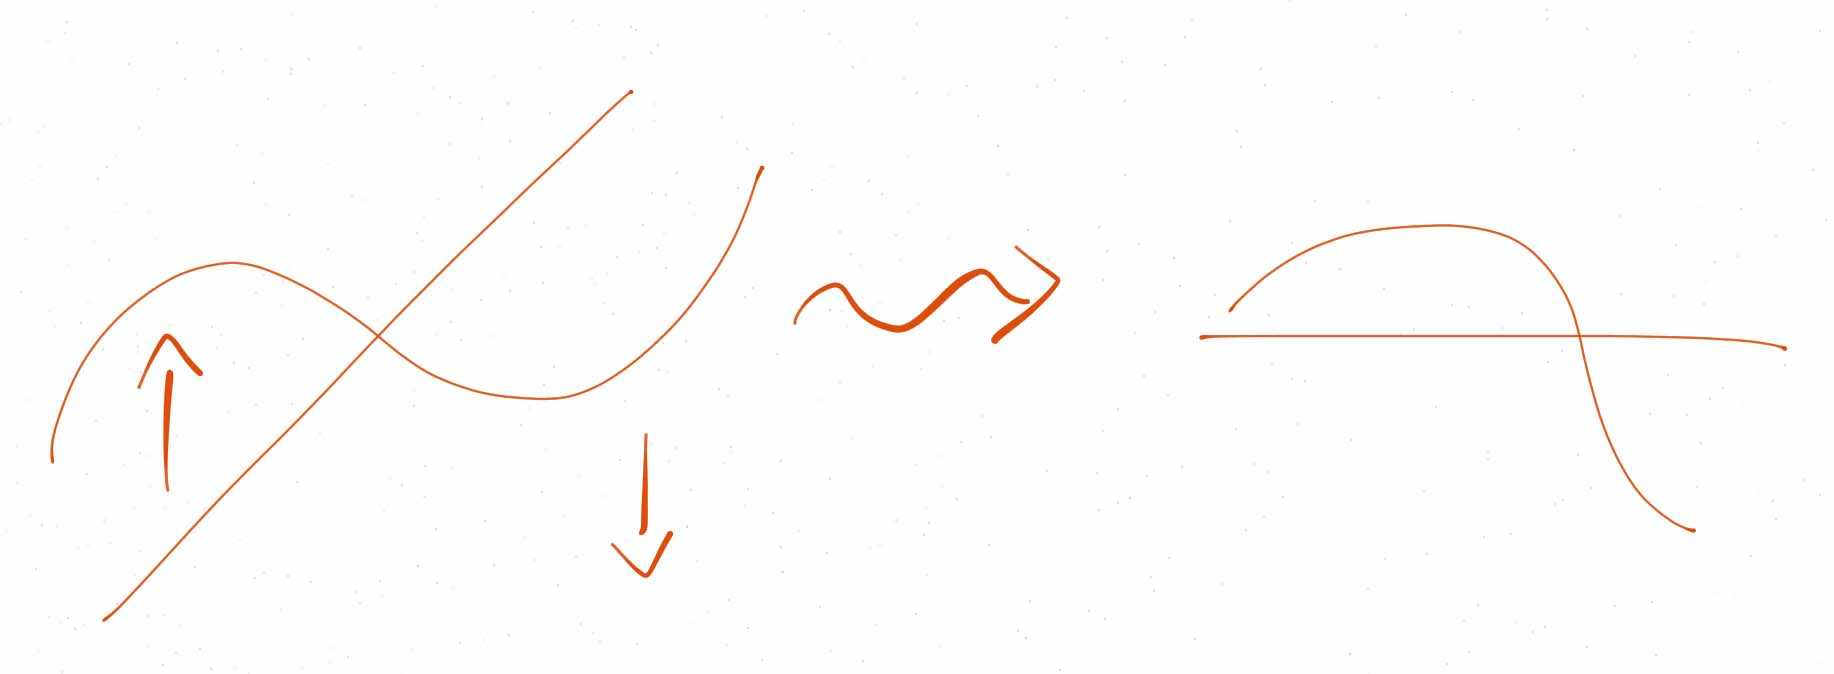
\includegraphics[width = 12cm]{rotate.jpg}
\end{center}

\begin{proof}
Set $g(x) = f(x) - x$, $g: [0,1] \to [0,1]$ is continuous. 

So $g(0) = f(0) - 0 \geq 0$, $g(1) = f(1) -1 \leq 0$

So by IVT $\exists x\in[0,1]$ s.t. $g(x) = 0\iff f(x) = x$	
\end{proof}

So if during the lecture you watch last weeks lecture on Panopto, using pause, fast-forward, rewind, play (but no jumping!) then at some point you will be watching a time in the lecture which equals the time now. (No matter where you start or end.) \\

\begin{definition}
	$S \subseteq \RR^n$,$f: S \to\RR$. Then we say that $f$ is bounded above if $\exists M \iR$ s.t. $f(\vec{x}) \leq M$ $\forall \vec{x} \in S$. 
	
	Similar for bounded below, bounded is both. 
\end{definition}

\begin{example}
$f(x) = \frac{1}{x}: (0,1] \to \RR$ is not bounded above

\begin{proof}
Suppose $\frac{1}{x} \leq M~\forall x\in(0,1]$ (Then $M > 0!$).
 
Then take $x = \mathrm{min}\{\frac{1}{2m},1) \implies x \leq 1/2m \implies 1/x \geq 2M > M,~\cont$.
\end{proof}	
\end{example}

Also $f(x) = \begin{cases}
 \frac{1}{x} & x\neq 0\\
 0 & x = 0	
 \end{cases}$
 
 $f:[0,1]\to \RR$ is also unbounded. Note that $f$ is not continuous at 0!
 
 So $\begin{cases}
	\mbox{discontinuous functions can be unbounded}\\
	\mbox{continuous functions can be unbounded on non-closed intervals}
\end{cases}$

But..

\begin{theorem}
$f:[a,b] \to \RR$ cts $\implies f$ is bounded.	
\end{theorem}

Ex: Give a function $f: [a,b] \cap \QQ \to \RR$ which is continuous and unbounded. 

\begin{proof}[Proof]\lecturemarker{23}{5 Oct}
Suppose not. Then $\forall N \in \mathbb{N}$, $N$ is not an unpperbound, so $\exists x_N \in [a,b]$ such that $|f(x_n)| > N$.

By BW Theorem, exists convergent subsequence, $y_i := x_{N(i)}, y_i \to y \in [a,b]$. With $|f(y_i)| = |f(x_{N(i)})| > N(i) \geq i ~(*)$. 

Fix $\epsilon =1$, then 
\[\exists \delta > 0\text{ such that }\forall x \in (y-\delta, y + \delta): |f(x) - f(y)| < 1 \implies |f(x)| < |f(y)| +1.\]
 Since $y_i \to y$, 
 \[\exists N\text{ such that }\forall n \geq N~ |y_n - y| < \delta \implies y_n \in (y-\delta, y + \delta) \implies |f(y_n)| < |f(y)| + 1.\]
 
 By $(*)$, $n \leq |f(y_n)| < |f(y)| + 1~ \forall n \geq N$, not true by the Archimedean Axiom $\cont$.
\end{proof}

\begin{proof}[Slicker Proof]
	Suppose not. Then $\forall N \in \mathbb{N}$, $N$ is not an unpperbound, so $\exists x_N \in [a,b]$ such that $|f(x_n)| > N$.
	
By BW Theorem, exists cvgt subsequence, $y_i := x_{N(i)}, y_i \to y \in [a,b]$. With $|f(y_i)| = |f(x_{N(i)})| > N(i) \geq i ~(*)$. $f$ is cts at $y \implies f(y_i) \to f(y)$, contradicting $(*)$.  
\end{proof}\vspace*{5pt}


\subsektion{Extreme Value Theorem}\vspace*{5pt}
\begin{theorem}[Extreme Value Theorem] $f: [a,b] \to \RR$ cts $\implies f$ bounded and attains its bounds.
\end{theorem}

So max $f(x)$ exists (not just sup)

\begin{proof}[Proof]
	By boundedness theorem, $\exists \displaystyle{\text{sup}_{x \in [a,b]}} f(x) = s$. Suppose for contradiction $\not \exists c \in [a,b]$ such that $f(x) = s$. 
	
	\emph{2 proofs}:
	
	(1) Then $s-f(x) > 0 ~\forall x \in [a,b],$ so $g(x) = \frac{1}{s-f(x)}: [a,b] \to \RR$ is well defined and cts. So $g(x)$ is bounded by $M > 0 \implies \frac{1}{s-f(x)} \leq M \implies f(x) \leq s - \frac{1}{M}$, so $s \neq$ sup$f(x),~\cont$.\vspace*{10pt}

	(2) From M1F $\exists$ a sequence $x_n \in [a,b]$ such that $f(x) \to  \displaystyle{\text{sup}_{x \in [a,b]}} f(x) = s$. BW Theorem $\implies$ exists subsequence $y_i := x_{N(i)}$ such that $y_i \to c \in [a,b].$ $f$ is cts $\implies f(y_i) \to f(x)$. Since $f(y_i) \to s$, by uniqueness of limits, $f(c) = s$.
	\end{proof}
	
	Combining IVT + EVT we get
	
	\begin{theorem}
	$f: [a,b] \to \RR$ is continuous then $\exists c,d \in [a,b]$ s.t. im$f = f[a,b]$ is the interval $[f(c),f(d)]$. 	
	\end{theorem}
	
	\begin{proof}
	EVT $\implies \exists c,d$ s.t. $f[a,b] \subseteq [f(c),f(d)] ~(*)$
	
	Given any $y \in [f(c),f(d)]$ the IVT $\implies \exists x$ between $c$ and $d$ s.t. $f(x) = y$, so $(*)$ is onto.	
	\end{proof}

\subsektion{Inverse Function Theorem}\vspace*{5pt}

\begin{proposition}
If $f:[a,b]\to\RR$ is continuous and strictly increasing ($x>y \implies f(x) > f(y)$), then $f$ is a bijection $[a,b] \to [f(a),f(b)]$	
\end{proposition}
\begin{proof}
$f(a)$ is a minimum of $f[a,b]$ because $x>a\implies f(x) > f(a)$. $f(b)$ is maximum. So by previous result $f[a,b] = [f(a), f(b)]$. We just need too show that $f$ is injective: 

If $x \neq y$, w.l.o.g. $x \neq y$ then $x < y \implies f(x) < f(y) \implies f(x) \neq f(y)$. So $f$ is injective. 
\end{proof}

So $\exists$ inverse $g := f^{-1}: [f(a),f(b)] \to [a,b]$

\begin{proposition}
$g$ is continuous (and also strictly increasing - Ex!)	
\end{proposition}

\begin{proof}
Fix $\epsilon >0$ and $y_0 \in [f(a),f(b)]$. 

Set $\delta:= \mathrm{min}(f(g(y_0) + \epsilon) - f(g(y_0)), f(g(y_0)) - f(g(y_0) - \epsilon))$

$ = \mathrm{min}(f(x_0 + \epsilon) -  y_0, y_0 - f(x-\epsilon))$	 where $x_0 = g(y_0)$

\emph{Picture:} 
\begin{center}
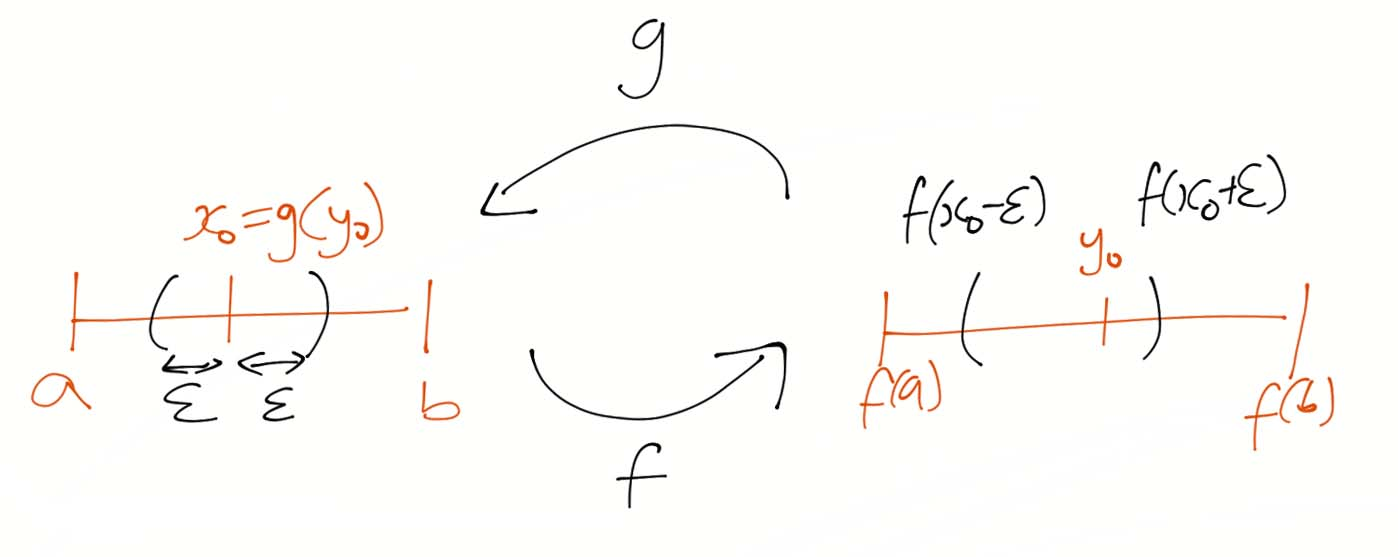
\includegraphics[width = 12cm]{ball2.jpg}
\end{center}

In this definition we use the convention that if $x_0 -\epsilon <a$ then by $f(x_) - \epsilon$ I mean $f(a)$ if $x_0 + \epsilon > b$ then $f(x_0 + \epsilon)$ means $f(b)$. 

(Equivalently I've extended $f$ to $\tilde f: \RR \to \RR$ by $\tilde f(x) =\begin{cases}
f(a) & x \leq a\\
f(x) & x \in [a,b]\\
f(b) & x \geq b
\end{cases}
$)

So $\delta$ was chosen s.t. $(y_0 -\delta, y_0 + \delta) \subseteq (f(x_0 - \epsilon), f(x+\epsilon))$, so $y \in (y_0 - \delta, y_0 + \delta) \cap [a,b]$ then $f(x_0 -\epsilon) < y < f(x_0 + \epsilon)$

Apply $g\implies x_0 -\epsilon < g(y) < x_0 + \epsilon$. Recall $x_0 = g(y_0) \implies |g(y) - g(y_0)| < \epsilon$.
\end{proof}

\begin{corollary}
$\sqrt{x}: [0,\infty) \to [0,\infty)$, $x^{1/n}: [0,\infty) \to [0,\infty),~n\iN$ are continuous. 	
\end{corollary}

Simpler exposition: Fix $f: \RR \to \RR$ bijective and continuous. Before we prove $f^{-1}$ is continuous we prove

\begin{lemma}\lecturemarker{24}{5 Oct}
$f:\RR \to \RR$ is bijective and cts $\implies f$ is strictly monotonic	
\end{lemma}

\begin{proof}
We prove this on any closed bounded interval $[a,b]$ (Hence monotonic on $\RR!$ Ex!)

$f$ is bijective, so $f(a) \neq f(b)$, w.l.o.g. $f(b) > f(a).$ Suppose for contradiction $\exists c \in (a,b)$ such that $f(c) \not\in (f(a),f(b)).$ 

w.l.o.g. take $f(c) > f(b)$. Then fix $d \in (f(b),f(c))$. By IVT applied to:
\begin{itemize} 
\item $f|_{[a,c]}$, we find $\exists x \in (a,c)$ such that $f(x) = d$. 
\item $f|_{[c,b]}$, we find $\exists y \in (c,b)$ such that $f(y) = d$.
	
\end{itemize}
But $y > x \implies x  \neq y$, so $f$ is not injective $\cont$. 

So $\forall c \leq b$, we find that $f(c) \leq f(b)$, and $f$ injective $\implies f(c) < f(b)$. 
\end{proof}\vspace*{5pt}

\begin{theorem}
	$f: \RR \to \RR$ bijective and cts $\implies f^{-1}: \RR \to \RR$ cts.
\end{theorem}
\begin{proof}
By Lemma $f$ is strictly monotonic, w.l.o.g. strictly increasing. 

We want to show $f^{-1}$ is continuous at $y\iR$. Let $x_0 \iR$ be $f^{-1}(y_0)$, so $f(x_0) = y_0$.

Fix $\epsilon > 0$.

Let $\delta :=$ min$\{f(x_0 + \epsilon) - y_0, y_0 - f(x_0 - \epsilon)\}$. 
 
 Then $|y -  y_0| < \delta \implies y \in (y_0 -\delta, y_0 + \delta) \subseteq (f(x_0 - \epsilon), f(x_0 + \epsilon))$. 
 
 Applying $f^{-1}$ preserves order \[\implies f^{-1}(y) \in (x_0 - \epsilon, x_0 + \epsilon) \iff |f^{-1}(y) - f^{-1}(y_0)| < \epsilon.\qedhere\]
\end{proof}\vspace*{5pt}

\begin{corollary}
$E:\RR \to \RR$, $E(x): \sum \frac{x^n}{n!}$ is a continuous bijection $\RR \to (0,\infty)$ with continuous inverse $\log: (0,\infty) \to \RR$. 	
\end{corollary}\vspace*{5pt}

We already showed that $E$ is continuous, never takes the value $0$ ($E(-x) = E(x)^{-1}$) is unboundedly poisitive for $x \geq 0$ ($E(x) \geq 1 + x$) and positive for $x < 0$ ($E(-x) = E(x)^{-1}$). So by IVT it takes \emph{every} value in $(0,\infty)$ (Ex!). 

We also showed it is strictly monotonically increasing ($E(y) = E(y-x)E(x) > E(x)$ for $y > x$). So by previous result it's a bijection to $(0,\infty)$ with a continuous inverse.\vspace*{5pt}


\begin{theorem}\lecturemarker{25}{12 March}
	$f:\RR^n \to \RR^m$ is cts at $\mathbf{a} = (a_1,\dots,a_n)$ if and only if $f_i:\RR^n \to \RR$ is cts at $a_i~\forall i$. (With $f = (f_1,\dots,f_m)$).
\end{theorem}

(i.e. $f_i$ is $\pi_i \circ f$ where $\pi_i: \RR^m \to \RR$ is the projection to the $i$th coordinate $\pi_i(x_1,\dots,x_m) = x_i$.)

\begin{proof}

Easy way is $\implies$:

\textsc{Highbrow:} $\pi_i: \RR^m \to \RR$ is continuous, so $\pi_i \circ f - f_i$ is continuous.

\textsc{First Principles:}
	Fix $\epsilon >0.$ Then $f$ is cts at $\vec{a} \implies \exists \delta >0 $ such that $|\vec{x} - \vec{a}| < \delta  \implies |f(\vec{x}) - f(\vec{a})| < \epsilon ~(*)$. But this implies $|f_i(\vec{x}) - f_i(\vec{a})| < \epsilon$ because
	
\[\begin{aligned}
|f(\vec{x}) - f(\vec{a})| &= \sqrt{\sum_{j=1}^m (f_j(\vec{x}) - f_j(\vec{a}))^2}\\
&\geq \sqrt{(f_i(\vec{x}) - f_i(\vec{a}))^2}\\
&= |f_i(\vec{x}) - f_i(\vec{a})| 	
\end{aligned}
\]	
\textsc{Proof of $\impliedby$:}

	Suppose $f_i$ cts at $a_i~\forall i$. Fix $\epsilon > 0$. Then $\exists \delta_i > 0$ such that \[|\vec{x} - \vec{a}| < \delta_i \implies |f_i(\vec{x}) - f_i(\vec{a})| < \epsilon\]
	 Set $\delta =$ min$\{(\delta_i\} >0$, so that 
	 \[\begin{aligned}|\vec{x} - \vec{a}| < \delta &\implies |f_i(\vec{x}) - f_i(\vec{a})| < \epsilon ~\forall i\\
	  \implies |f(\vec{x}) - f(\vec{a})| &= \sqrt{\sum_{i=1}^m (f_i(\vec{x}) - f_i(\vec{a}))^2} \\
	  &\leq \sqrt{\sum_{i=1}^m \epsilon^2} = \sqrt{m}.\epsilon	
\end{aligned}
\]
\end{proof}

So we can study the continuity of $f: \RR^n \to \RR^m$ in terms of their coordinates $f_i$ in $\RR^m$. But \emph{not} in terms of the restoration of $f$ to coordinate axises in $\RR^n$.\vspace*{15pt}

\begin{example}
$f: \RR^2 \to \RR$, $f(x,y) = \begin{cases}
 	\dfrac{xy}{x^2 + y^2} & (x,y) \neq (0,0)\\
 	0 & (x,y) = (0,0)
 \end{cases}$
 
 On any horizontal line $y =c$ it results to the function 
 \[f(x,c) = \frac{cx}{c^2 + x^2} \quad \text{ if } c \neq 0\]
 \[\text{ or } f(x,0) \equiv 0 ~\forall x \quad \text{ if } c = 0\]
 Both are continuous functions $\RR \to \RR$. 
 
 Similarly on any vertical line $x = c$, $f$ restricts to a continuous function: 
  \[f(c,y) = \frac{cy}{c^2 + y^2} \quad \text{ if } c \neq 0\]
 \[\text{ or } f(0,y) \equiv 0 ~\forall y \quad \text{ if } c = 0\]
 But $f$ is \emph{not} continuous at $(0,0)$
 
 \emph{Idea:} on line $y=x$, $f$ is $\begin{cases}
	\dfrac{x.x}{x^2 + x^2} = \frac{1}{2} & \forall x \neq 0\\
	0 & x = 0
\end{cases}$

Pick $\epsilon = \frac{1}{2}$. Then for any $\delta > 0$, take $x = \frac{\delta}{2}$ so that $(x,x) \in B_\epsilon(0,0)$. But $f(x,x) = \frac{1}{2} \not\in B_\epsilon(f(0,0)) = B_\epsilon(0)$. So $f$ is not continuous at $(0,0)$. \qed
\end{example}

Ex: Converse is true: if $f: \RR^n \to \RR^m$ is continuous then $f$ is continuous on restriction to any line in $\RR^n$; more generally $\left.f\right|_S: S \to \RR^m \text{ is continuous } \forall S \subseteq \RR^n$



